% GO TO: /Users/leonlufkin/Library/texmf/tex/latex
%        to add custom packages to the path
\documentclass{article}
\usepackage{report}

\title{Making Things Precise}
\author{Leon Lufkin}
\date{\today}

\makeatletter
\let\Title\@title
\let\Author\@author
\let\Date\@date

\begin{document}

%%%%%%%%%%%%%
%% Setting %%
%%%%%%%%%%%%%
\section{Setting}
We are interested in characterizing the structure learned in the first layer of a deep neural network when trained on a simple task.

\paragraph*{Data}
In the most general case, our data are sampled from zero-mean stochastic processes defined on the probability space $(\Omega, \FF, p)$ with values in the measurable space $(\R, S)$.
The measure $p$ is parameterized by $\xi > 0$, which controls the length-scale of the correlations, and $g > 0$, which controls the degree of non-Gaussianity.
(I'm not sure how to rigorously add more structure to this.)
A single realization of this stochastic process is denoted by $X(t)$.

Informally, $\xi$ controls the frequency of oscillations\footnote{``Oscillation'' isn't the right word, but $\xi$ certainly controls the number of times $X(t)$ crosses zero, which is what I mean by frequency.
Importantly, this definition of ``frequency'' is invariant to $g$!
(Note that the correlation between two points is not invariant to choice of $g$, so this might actually be a useful definition.)} in $X(t)$, but it is important to note that $X(t)$ is not actually periodic.
See \Cref{fig:samples} for some samples.

As $g \to 0$, $X(t)$ converges in distribution to a Gaussian process with covariance function $\Sigma(\xi)(x,x')$.
As $g$ increases, $X(t)$ becomes increasingly non-Gaussian\footnote{What does this mean, exactly? If it's like what Alessandro did, then it means super-Gaussian tails, kind of.}.

We take our index set to be $\Omega = \T^d$, the $d$-dimensional torus, so that our samples are periodic.
This naturally introduces Fourier series\footnote{But do we need them?}.

\begin{figure}[!h]
  \centering
  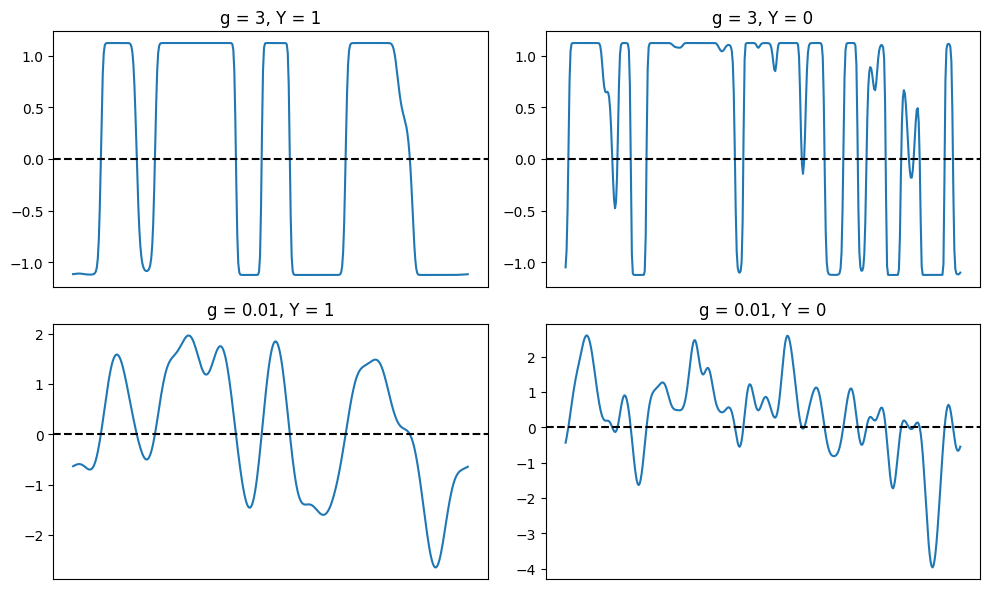
\includegraphics[width=0.8\textwidth]{figs/samples.png}
  \caption{1-$d$ samples $X(t)$ from discretization with $n = 400$, $(\xi_1, \xi_0) = (20, 10)$.}
  \label{fig:samples}
\end{figure}

\paragraph*{Model}
Our model is a two-layer neural network with $K$ hidden neurons and activation function $\sigma$.
\begin{align}
  \hat{y}(x) &= \frac{1}{K} \sum_{k\in[K]} \sigma( \langle w_k, x \rangle + b_k ).
\end{align}
We call $w_k$ the receptive field (RF) of the $k$-th neuron and $b_k$ its bias.
Here, $\langle w_k, x \rangle = \int_{\T^d} w_k(t) x(t) dt$.

\paragraph*{Objective}
The task is to discriminate which of two processes $\{ X_1(t) \}$ and $\{ X_0(t) \}$, parameterized by $\xi_1$ and $\xi_0$, respectively, for some fixed $g$, a given sample $X(t)$ was drawn from.
If the former, the desired label is $Y_1$, otherwise it is $Y_0$.
So, we seek weights $\{ w_k, b_k \}_{k\in[K]}$ that minimize the loss
\begin{align}
  \LL &= \frac{1}{2} \E_{X,Y} \left[ \left( \hat{y}(X) - Y \right)^2 \right]. \label{eq:loss}
\end{align}

\paragraph*{Practice}
I've presented a very general version of the problem we have to strip away what I deem irrelevant details.
However, in practice, we must add many more constraints.

First, we cannot train continuous RFs or sample from arbitrary stochastic processes.
So, we restrict $\Omega$ to the finite set $\{ \frac{i}{n} \mid 0 \leq i < n \}^d \subseteq \T^d$.
In fact, we typically just take $d=1$.
So, $X(t)$ and $w_k$ are vectors in $\R^n$.
The inner product simplifies to the standard Euclidean inner product.

Secondly, we tune $w_k$ and $b_k$ using full-batch stochastic gradient descent, which is not guaranteed to minimize the loss in \cref{eq:loss}.


%%%%%%%%%%%%%%%%%%%%%%%%%
%% Functional Behavior %%
%%%%%%%%%%%%%%%%%%%%%%%%%
\section{Functional Behavior}
While analyzing this model exactly is nearly impossible, its functional behavior is quite easy to understand.
We will consider sigmoid activation because it yields both oscillatory and localized RFs.
We'll start by simplifying the model's structure a bit before explaining exactly how it solves the task.

\subsection*{Reducing the model}

\paragraph*{Frequency specialization}
With sigmoid activation, the model learns to solve the task by creating two populations of neurons roughly in equal size, one with RFs resembling localized weights (or long-range oscillations) and the other with RFs resembling short-range oscillations.
We call this \emph{frequency specialization}.

We'll attach the label $-$ to the former and $+$ to the latter.
(This is because the former learns negative bias terms, while the latter learns positive ones.
More on this later.)
The biases within each class are all approximately the same.
So, we'll reduce our model to
\begin{align}
  \hat{y}(x) &= \frac{1}{K} \bigg( \underbrace{ \sum_{k\in[-]} \sigma( \langle w_k, x \rangle + b^- ) }_\text{localized} + \underbrace{ \sum_{k\in[+]} \sigma( \langle w_k, x \rangle + b^+ ) }_\text{oscillatory} \bigg).
\end{align}

The facts that it constructs two populations of neurons and that they are equal in size seems to be arbitrary.
It appears that either population could solve the task on its own, and balancing is not required.

[insert figure showing unbalanced classes]

(TODO: Test if just oscillatory neurons can do the task!)
[insert figure showing just localized (and perhaps just oscillatory) solve the task]

\paragraph*{Tiling}
In addition to the biases being approximately the same within each class, the RFs also exhibit a lot of symmetry.
Within each class, the RFs differ only in where they are centered (for long-range neurons, at least) and their sign.
That is, they implement a high-degree of \emph{weight sharing} and \emph{tile} the input space.
As we increase $K$, the number of hidden neurons, to be very large, they effectively implement a convolution (but the integrand is wrapped by $\sigma$).
We further reduce our model to
\begin{align}
  % \hat{y}(x)
  % &= \frac{1}{2} \bigg( \int_{\T} \sigma( \langle w^-(\cdot - \tau), x \rangle + b^- ) d \tau + \int_{\T} \sigma( \langle w^+(\cdot - \tau), x \rangle + b^+ ) d \tau \bigg) \\
  \begin{multlined} 
    \hat{y}(x) =\frac{1}{4} \bigg( 
      \underbrace{ \int_{\T} \sigma( ( w^- * x )(\tau) + b^- ) d \tau + \int_{\T} \sigma( -( w^- * x )(\tau) + b^- ) d \tau }_\text{localized} +  \\
      \underbrace{ \int_{\T} \sigma( ( w^+ * x )(\tau) + b^+ ) d \tau + \int_{\T} \sigma( -( w^+ * x )(\tau) + b^+ ) d \tau }_\text{oscillatory} 
    \bigg). \label{eq:reduced_model}
  \end{multlined}
\end{align}
Note that when $( w^- * x )(\tau) + b^-$ is large enough to be significant in the sigmoid, then $-( w^- * x )(\tau) + b^-$ is extremely small and thus insignificant. 
So, we can reduce the first two terms by considering just $|( w^- * x )(\tau)| + b^-$.
The same holds for $w^+$.
Thus,
\begin{align}
  \hat{y}(x)
  % &= \frac{1}{2} \bigg( \int_{\T} \sigma( \langle w^-(\cdot - \tau), x \rangle + b^- ) d \tau + \int_{\T} \sigma( \langle w^+(\cdot - \tau), x \rangle + b^+ ) d \tau \bigg) \\
  &= \frac{1}{2} \bigg( 
      \underbrace{ \int_{\T} \sigma( |( w^- * x )(\tau)| + b^- ) d \tau }_\text{localized} + 
      \underbrace{ \int_{\T} \sigma( |( w^+ * x )(\tau)| + b^+ ) d \tau }_\text{oscillatory} 
    \bigg). \label{eq:reduced_model}
\end{align}


\paragraph*{Localization}
The final phenomenon we observe is that $w^-$ is highly localized, while $w^+$ is not.
% Intuitively, this makes sense, but I'll explain this in more detail later.
To try to explain this, we'll consider how the model solves the task.
Let's just focus on $w^-$ for now.
We want $w^-$ to be structured so that it yields outputs closer to 1 upon observing data from $p_{\xi_1}$ and -1 otherwise (assuming $\sigma(x) = \operatorname{erf}(\frac{x}{\sqrt{2}})$).
Ideally,
\begin{align}
  \PR_{X_1, X_0} \left( \int \sigma( |(w^- * X_1)(\tau)| + b^- ) d \tau > \int \sigma( |(w^- * X_0)(\tau)| + b^- ) d \tau \right) \approx 1, \label{eq:optimal_RF_condition}
\end{align}
where the probability is over independent draws $X_1 \sim p_{\xi_1}$ and $X_0 \sim p_{\xi_0}$.
This condition is equivalent to having $w^-$ \emph{maximize the spread in the preactivations corresponding to $p_{\xi_1}$ relative to those for $p_{\xi_0}$}.
I'll explain why this is true now.

In the context of \cref{eq:optimal_RF_condition}, let's define the optimal RF $w^-$ as
\begin{align*}
  w^- &\triangleq \argmax_{w}  \PR_{X_1, X_0} \left( \int \sigma( |(w * X_1)(\tau)| + b^- ) d \tau > \int \sigma( |(w * X_0)(\tau)| + b^- ) d \tau \right).
\end{align*}
Considering independent uniform draws $\tau,\tau'$ from $\T$, we can (I think) rewrite this as
\begin{align}
  w^-
  &= \argmax_{w} \PR_{X_1, X_0, \tau, \tau'} \left( \sigma( |(w * X_1)(\tau)| + b^- ) > \sigma( |(w * X_0)(\tau')| + b^- ) \right) \label{eq:split_integral} \\
  &= \argmax_{w} \PR_{X_1, X_0, \tau, \tau'} \left( |(w * X_1)(\tau)| >  |(w * X_0)(\tau')| \right) && \text{monotonicity} \label{eq:single_term} \\
  &= \argmax_{w} \PR_{X_1, X_0} \left( |\langle w, X_1 \rangle| > |\langle w, X_0 \rangle| \right), && \text{translation invariance} \label{eq:spread_l1} \\
  &= \argmax_{w} \PR_{X_1, X_0} \left( (\langle w, X_1 \rangle)^2 > (\langle w, X_0 \rangle)^2 \right), \label{eq:spread_l2} 
\end{align}
\Cref{eq:spread_l1,eq:spread_l2} are obviously equivalent, but \cref{eq:spread_l2} just makes it a bit clearer that we want to think about the \emph{spread} of the preactivations.
Both $\langle w, X_1 \rangle$ and $\langle w, X_0 \rangle$ are symmetric, zero-mean random variables.
So, we cannot try to maximize the difference in their means.
However, because we have a (learnable) bias term, we can exploit the difference in their variances.
Specifically, we want to maximize the variance of $\langle w, X_1 \rangle$ relative to that of $\langle w, X_0 \rangle$.

\subsection*{Understanding the model}
\Cref{eq:spread_l1} gives us a reduced model to understand the optimization problem the model is solving.
Now, let's try to understand how it might solve this problem.
First, a caveat.

%% A cheat
\paragraph*{A cheat}
In moving from \cref{eq:split_integral} to \cref{eq:single_term}, we made the assumption that $b^-$ was fixed.
In practice, we tune $b^-$ along with $w^-$.
So, if the model is able to achieve \emph{some} advantage in \cref{eq:spread_l1}, it can just increase the norms of $w$ and $b^-$ to achieve a larger advantage in \cref{eq:single_term}.
This is a perfectly valid strategy, and one I would expect it to exploit.
This yields an important question: \emph{Does the model take the easy route by scaling up $w$, or does it properly optimize $w$?}

Empirically, we see that the norms of $w^-$ and $b^-$ do indeed grow throughout training.
The shape of the RF $w^-$ emerges relatively early on in training before it is ``smoothed out'' and scaled up in norm.

[TODO: insert plots showing this transition between the two states]

%% Gaussian data
\paragraph*{Gaussian data}
Let's momentarily assume $X_1$ and $X_0$ are Gaussian (i.e. $g \approx 0$) and go back to discrete land (it's a bit easier for my brain).
Then, $\langle w, X_i \rangle \sim \NN\left( 0, w^\top \Sigma_i w \right)$.
Recall that $X_1$ and $X_0$ are drawn independently.
So,
\begin{align*}
  \PR_{X_1, X_0} \left( |\langle w, X_1 \rangle| > |\langle w, X_0 \rangle| \right)
  &= \int_{\R} \int_{[-|x_1|,|x_1|]} p_0(x_0) p_1(x_1) dx_0 dx_1 \\
  &= \int_{\R} \left[ \Phi\left( \frac{|x_1|}{\sqrt{w^\top \Sigma_0 w}} \right) - \Phi\left( \frac{-|x_1|}{\sqrt{w^\top \Sigma_0 w}} \right) \right] p_1(x_1) dx_1 \\
  % &= 2 \int_{\R_{\geq 0}} \left[ 2 \Phi\left( \frac{x_1}{\sqrt{w^\top \Sigma_0 w}} \right) - 1 \right] p_1(x_1) dx_1 \\
  % &= 4 \int_{\R_{\geq 0}} \Phi\left( \frac{x_1}{\sqrt{w^\top \Sigma_0 w}} \right) p_1(x_1) dx_1 - 1 \\
  % &= 4 \int_{\R_{\geq 0}} \left[ \frac{1}{2} \operatorname{erf}\left( \frac{1}{\sqrt{2}} \cdot \frac{x_1}{\sqrt{w^\top \Sigma_0 w}} \right) + \frac{1}{2} \right] p_1(x_1) dx_1 - 1 \\
  &= 2 \int_{\R_{\geq 0}} \operatorname{erf}\left( \frac{1}{\sqrt{2}} \cdot \frac{x_1}{\sqrt{w^\top \Sigma_0 w}} \right) p_1(x_1) dx_1 \\
  % &= \frac{ 2 }{ \sqrt{2\pi} \cdot \sqrt{w^\top \Sigma_1 w} } \int_{\R_{\geq 0}} \operatorname{erf}\bigg( \underbrace{ \frac{1}{\sqrt{2 (w^\top \Sigma_0 w)}} }_{\triangleq a} x_1 \bigg) \exp\bigg( - \underbrace{\frac{1}{2 (w^\top \Sigma_1 w)}}_{\triangleq b^2} x_1^2 \bigg) dx_1 \\
  % &= \frac{ 2 }{ \sqrt{(2 \pi) w^\top \Sigma_1 w} } \left[ \frac{\sqrt{\pi}}{2b} - \frac{1}{b \sqrt{\pi}} \tan^{-1}\left( \frac{b}{a} \right) \right] \\
  &= 1 - \frac{2}{\pi} \tan^{-1} \left( \sqrt{ \frac{ w^\top \Sigma_0 w }{ w^\top \Sigma_1 w } } \right).
\end{align*}
Therefore, for Gaussian data,
\begin{align*}
  w^- 
  &= \argmax_{w \in S^{n-1}} \PR_{X_1, X_0} \left( |\langle w, X_1 \rangle| > |\langle w, X_0 \rangle| \right) \\
  &= \argmax_{w \in S^{n-1}} 1 - \frac{2}{\pi} \tan^{-1} \left( \sqrt{ \frac{ w^\top \Sigma_0 w }{ w^\top \Sigma_1 w } } \right) \\
  &= \argmin_{w \in S^{n-1}} \frac{ w^\top \Sigma_0 w }{ w^\top \Sigma_1 w } \\
  &= F \left( \argmin_{u \in S^{n-1}} \frac{ u^\top \Lambda_0 u }{ u^\top \Lambda_1 u } \right),
\end{align*}
where $F$ is our real DFT operator and $\Lambda_i$ is the corresponding diagonal matrix of eigenvalues of $\Sigma_i$.
Again, we can take $u$ to be unit norm without loss of generality.
Then, $u^\top \Lambda_0 u = \sum_{k \in [n]} c_k \lambda_0^{(k)}$, where $c_k \geq 0$ and $\sum_k c_k = 1$.


%% Polar coordinates
\paragraph*{Polar coordinates}
Going back to discrete land, we can write the inner product in terms of the norm of $w$ and the angle between $w$ and $X_i$.
Starting from \cref{eq:spread_l1},
\begin{align}
  w^-
  &= \argmax_{w} \PR_{X_1, X_0} \left( |\cos \theta(w,X_1) | \norm{X_1}_{2} > | \cos \theta(w,X_0) | \norm{X_0}_{2} \right) \\
  &= \argmax_{w} \PR_{X_1, X_0} \left( \frac{ |\cos \theta(w,X_1) | }{ | \cos \theta(w,X_0) | } > \frac{ \norm{X_0}_{2} }{ \norm{X_1}_{2} } \right)
\end{align}
We cannot control the norms on the right side of the inequality.
So, we need to construct $w$ to maximize the left side.
We do this by making $w$ be as parallel to $X_1$ as possible while making it as orthogonal as possible to $X_0$\footnote{We haven't really said anything new here—this is already apparent in \cref{eq:spread_l1,eq:spread_l2}.}.

%% Fourier space
\paragraph*{Fourier space}
Returning to the continuous realm, we use Parseval's theorem\footnote{This says the Fourier transform is unitary from $L^2(\T)$ to $\ell^2(\Z)$. The result for DFT is analogous.} to rewrite \cref{eq:spread_l1}
\begin{align}
  w^-
  &= \argmax_{w} \PR_{X_1, X_0} \left( |\langle \FF w, \FF X_1 \rangle| > |\langle \FF w, \FF X_0 \rangle| \right), \\
  &= \argmax_{\widehat{w}} \PR_{\widehat{X}_1, \widehat{X}_0} \left( |\langle \widehat{w}, \widehat{X}_1 \rangle| > |\langle \widehat{w}, \widehat{X}_0 \rangle| \right).
\end{align}
All we've done is represent the problem in Fourier space.
I'm not sure if this is actually helpful.

%% Difference in means
\paragraph*{Difference in means}
It's hard to make a ton of analytical progress here, so we'll have to defer to simulations (for now).
We can, though, compute the means of the squared terms in \cref{eq:spread_l2}.
For $i=0,1$,
\begin{align*}
  \E_{X_i} \left[ (\langle w, X_i \rangle)^2 \right]
  &= \E_{X_i} \left[ \left( \int_{\T} w(s) X_i(s) ds \right) \left( \int_{\T} w(t) X_i(t) dt \right) \right] \\
  &= \int_{\T} \int_{\T} w(s) w(t) \E_{X_i} \left[ X_i(s) X_i(t) \right] ds dt \\
  &= \int_{\T} \int_{\T} w(s) w(t) k_i(s,t) ds dt \\
  &= \langle K_i w, w \rangle_{L^2},
\end{align*}
where $K_i w(t) = \int_{\T} k_i(s,t) w(s) ds$.
Therefore,
\begin{align*}
  \E_{X_1} \left[ (\langle w, X_1 \rangle)^2 \right]
  - \E_{X_0} \left[ (\langle w, X_0 \rangle)^2 \right]
  &= \langle K_1 w, w \rangle_{L^2} - \langle K_0 w, w \rangle_{L^2} \\
  &= \langle (K_1 - K_0) w, w \rangle_{L^2}.
\end{align*}
Note that the probability in \cref{eq:spread_l2} is invariant to scaling $w$.
So, let's fix $\norm{w}_{L^2} = 1$.
Then, maximizing this is just finding the leading eigenvector of the operator $K_1 - K_0$.
% Going back to discrete land, this is the same as finding the leading eigenvector of the $n \times n$ matrix $\Sigma_1 - \Sigma_0$.
% Recall that $\Sigma_0$ and $\Sigma_1$ are real, circulant, symmetric matrices, so $\Sigma_1 - \Sigma_0$ is as well.
% Then, their eigenvalues are given by
% \begin{align}
%   \frac{\lambda_j }{n}
%   &= \frac{1}{n} \sum_{k=0}^{n-1} (\Sigma_1 - \Sigma_0)_{1,k} \re( e^{2 \pi i \frac{j k}{n}} ) \\
%   &= \frac{1}{n} \sum_{k=0}^{n-1} \left( e^{ -\frac{k^2}{\xi_1^2 n^2} } - e^{ -\frac{k^2}{\xi_0^2 n^2} } \right) \cos( 2 \pi \tfrac{j k}{n} ) \\
%   &\to \int_{\T} \left( e^{ -\frac{x^2}{\xi_1^2} } - e^{ -\frac{x^2}{\xi_0^2} } \right) \cos( 2 \pi j x ) dx
%   \triangleq A.
% \end{align}
% We want to optimize this over $j$.
% Using DCT, the optimality condition is
% \begin{align*}
%   0 = \frac{ \partial A }{ \partial j } &= \int_{\T} \left( e^{ -\frac{x^2}{\xi_1^2} } - e^{ -\frac{x^2}{\xi_0^2} } \right) (-2 \pi x) \sin( 2 \pi j x ) dx.
% \end{align*}
We can show that this is the constant function, which is inconsistent with our observation that we get Gabor-like RFs.
Let's test this result empirically to see has any merit (note that maximizing the difference in means is \emph{not} the same as maximizing the probability dominance), and if Gabors are actually better.

\subsection*{Optimality}
We've explored what it takes for our neural network model to be optimal, but we want to understand how close it gets to universal optimality.
We'll consider accuracy instead of loss because it lets us invoke the Neyman-Pearson lemma.

Let us start by considering an arbitrary classifier $\hat{y}$ that sends an input $X_i$ to either $0$, if it believes $X_i \sim p_{\xi_0}$, or $1$ otherwise.
Then, the optimal classifier, in terms of accuracy, is
\begin{align*}
  \hat{y}^* = \argmax_{\hat{y}} \PR_{X_1,X_0}( \hat{y}(X_i) = i )
\end{align*}
We can pose this as a hypothesis testing problem.
\begin{align*}
  H_0 &: X \sim p_{\xi_0} \\
  H_1 &: X \sim p_{\xi_1}
\end{align*}
The Neyman-Pearson lemma tells us that the likelihood ratio test has the largest accuracy\footnote{Note that $1 - $accuracy = Type 1 error $+$ Type II error, which the likelihood ratio test minimizes.} among all tests.
That is,
\begin{align*}
  \hat{y}^*(x) &= 
  \begin{cases}
    1 & \text{if } L(x) \triangleq \frac{ p_{\xi_1}(x) }{ p_{\xi_0}(x) } > \eta \\
    0 & \text{otherwise}  
  \end{cases},
\end{align*}
for some threshold $\eta > 0$.
The corresponding accuracy is
\begin{align*}
  \frac{1}{2} \left( \PR_{X_1}\left( L(X_1) > \eta \right) + \PR_{X_0} \left( L(X_0) \leq \eta \right) \right)
  % &= 1 - \PR_{X_1,X_0}\left( L(X_1) \leq \eta \land L(X_0) > \eta \right) \\
  % &= 1 - \PR_{X_1,X_0}\left( L(X_1) \leq \tau < L(X_0) \right).% \\
  % &= \PR_{X_1,X_0}\left( L(X_1) \geq \tau > L(X_0) \right).
\end{align*}
% Note this is invariant to $\tau$.

I think we can make some progress here for the general case, but let's just consider Gaussian data for now.

\paragraph*{Gaussian data}
\begin{align*}
  \frac{ p_{\xi_1}(x) }{ p_{\xi_0}(x) }
  &= \frac{ \frac{1}{(2\pi)^{n/2}} |\Sigma_1|^{-\frac{1}{2}} \exp \left( -\frac{1}{2} x^\top \Sigma_1^{-1} x \right) }{ \frac{1}{(2\pi)^{n/2}} |\Sigma_0|^{-\frac{1}{2}} \exp \left( -\frac{1}{2} x^\top \Sigma_0^{-1} x \right) } \\
  &= \sqrt{ \frac{|\Sigma_0|}{|\Sigma_1|} } \exp \left( -\frac{1}{2} x^\top (\Sigma_1^{-1} - \Sigma_0^{-1}) x \right) \\
  &\simeq x^\top (\Sigma_1^{-1} - \Sigma_0^{-1}) x,
\end{align*}
where $\simeq$ means equal up to some monotonic transformation.
% Let's further write this by diagonalizing the covariance matrices in the real DFT basis.
% Letting $u = P^\top x$,
% \begin{align*}
%   \frac{ p_{\xi_1}(x) }{ p_{\xi_0}(x) }
%   &\simeq u^\top (\Lambda_1^{-1} - \Lambda_0^{-1}) u.
% \end{align*}
% So, we want to find the threshold $\eta$ such that the test
% \begin{align*}
%   \hat{y}^*(x) &= 
%   \begin{cases}
%     1 & \text{if } u^\top (\Lambda_1^{-1} - \Lambda_0^{-1}) u < \eta \\
%     0 & \text{otherwise}  
%   \end{cases},
% \end{align*}
% has greatest accuracy.

So, the optimal accuracy is given by
\begin{align*}
  \min_{\eta > 0} \frac{1}{2} \left( \PR_{X_1}\left( X_1^\top (\Sigma_1^{-1} - \Sigma_0^{-1}) X_1 < \eta \right) + \PR_{X_0} \left( X_0^\top (\Sigma_1^{-1} - \Sigma_0^{-1}) X_0 \geq \eta \right) \right)
\end{align*}


\paragraph*{Non-Gaussian data}



% \subsection*{Understanding the model}
% \Cref{eq:reduced_model} gives us a simple model to understand.
% We've said that $b^-$ is negative and $b^+$ is positive, but does this have to be the case?

% Assume for a moment that $b^- = b^+ = 0$.
% The true labels are invariant to sign-flips of the input, but the preactivations $( w^- * x )(\tau)$ and $( w^+ * x )(\tau)$ are not—they are equivariant to sign-flips.
% For an even activation like sigmoid, if the biases $b^-$ and $b^+$ are zero, then the postactivations, and thus the predicted labels, will be equivariant to sign flips of the input as well.
% This is not what we want.

% We can fix this by making the bias terms nonzero, or by choosing a non-even activation function.
% We'll consider the former for now, but the latter is the reason why ReLU activation works without a bias term.

% Given nonzero bias terms, how does the model solve the task?
% Recall that the pre-bias pre-activations are equivariant to sign-flips of the input.
% So, they'll always have mean zero, which means the model has to learn to manipulate the spread of preactivations to solve the task.

% We'll explain how it does this by starting with the observation that the RF $w^-$ has a longer frequency\footnote{Recall our loose definition from earlier, where we define the ``frequency'' of an input signal in terms of how many times it crosses zero. For RFs, because of Fourier components, we can use this term more rigorously.} than $w^+$.
% So, if our input is sampled from the long-range correlation class, $X(t) \sim p_{\xi_1}$, then we want $( w^- * X )(\tau)$ to have a larger spread so that more values will be positive and $\sigma( ( w^- * X )(\tau) + b^- )$ will, on average, be larger.
% \emph{This has translated a second-moment change into a first-moment change.}

% \begin{align}
%   ( w^- * X )(\tau)
%   % &= \FF^{-1}( \{ \widehat{( w^- * X )}(n) \}_{n \in \Z} )(\tau)
%   &= \sum_{n \in \Z} \widehat{( w^- * X )}(n) e^{2\pi i n \tau} \\
%   &= \sum_{n \in \Z} \widehat{w^-}(n) \widehat{X}(n) e^{2\pi i n \tau}
% \end{align}

% \begin{align}
%   \E_X\left[ ( w^- * X )(\tau) \right] &= 0
% \end{align}

% \begin{align}
%   \E_X\left[ ( w^- * X )^2(\tau) \right]
%   &= \E_X\left[ \left( \sum_{n \in \Z} \widehat{w^-}(n) \widehat{X}(n) e^{2\pi i n \tau} \right) \left( \sum_{m \in \Z} \widehat{w^-}(m) \widehat{X}(m) e^{2\pi i m \tau} \right) \right] \\
%   % &= \E_X\left[ \sum_{n \in \Z}  \sum_{m \in \Z} \widehat{w^-}(n) \widehat{X}(n) \widehat{X}(m) e^{2\pi i (n+m) \tau} \widehat{w^-}(m) \right] \\
%   &= \sum_{(m,n) \in \Z^2} \widehat{w^-}(m) \widehat{w^-}(n) \E_X\left[ \widehat{X}(m) \widehat{X}(n) \right] e^{2\pi i (m+n) \tau}
% \end{align}
% $\E_X [ \widehat{X}(n) \widehat{X}(m) ]$ is the covariance between the $n$-th and $m$-th Fourier coefficients of $X(t)$.
% Note that it is independent of $\tau$.

% \begin{align}
%   \E_X \left[ \widehat{X}(m) \widehat{X}(n) \right]
%   % &= \int_{\R} 
%   &= \E_X \left[ \left( \int_{\T} X(s) e^{-2 \pi i m s} ds \right) \left( \int_{\T} X(t) e^{-2 \pi i n t} dt \right) \right] \\
%   &= \int_{\T^2} \E_X \left[ X(s) X(t) \right] e^{-2 \pi i m s} e^{-2 \pi i n t} ds dt \\
%   &= \int_{\T^2} k(s,t) e^{-2 \pi i m s} e^{-2 \pi i n t} ds dt \\
%   &= \widehat{k}(m,n),
% \end{align}
% where $k$ is the covariance function for our stochastic process.
% Thus,
% \begin{align}
%   \E_X\left[ ( w^- * X )^2(\tau) \right]
%   &= \sum_{(m,n) \in \Z^2} \widehat{w^-}(m) \widehat{w^-}(n) \widehat{k}(m,n) e^{2\pi i (m+n) \tau} \\
%   &= \sum_{m \in \Z} \widehat{w^-}(m) e^{2\pi i m \tau} \sum_{n \in \Z} \widehat{w^- * k(m, \cdot)}(n) e^{2\pi i n \tau} \\
%   &= \sum_{m \in \Z} \widehat{w^-}(m) e^{2\pi i m \tau} w^- * k(m, \cdot)
% \end{align}

% Note
% \begin{align}
%   \E_X\left[ ( w^- * X )^2(\tau) \right]
%   &= \E_X\left[ \left( \int_{\T} w^-(s-\tau) X(s) ds \right) \left( \int_{\T} w^-(t-\tau) X(t) dt \right) \right] \\
%   &= \E_X\left[ \int_{\T^2} X(s) X(t) w^-(s-\tau) w^-(t-\tau) ds dt \right] \\
%   &= \int_{\T^2} \E_X\left[ X(s) X(t) \right] w^-(s-\tau) w^-(t-\tau) ds dt && \text{DCT} \\
%   &= \int_{\T^2} k(s,t) w^-(s-\tau) w^-(t-\tau) ds dt \\
%   &= \int_{\T^2} k(s-\tau,t-\tau) w^-(s-\tau) w^-(t-\tau) ds dt && \text{translation invariance} \\
%   &= \int_{\T^2} k(s,t) w^-(s) w^-(t) ds dt. && \text{$u$-sub}
%   % &= \norm{ w^- }_{k}^2.
%   % &= \langle k s, s \rangle.
% \end{align}
% This is a quadratic form, so we can diagonalize it.
% Note that it is invariant to $\tau$ (this makes intuitive sense).

% Intuitively, we wish to maximize $\E_X\left[ ( w^- * X )^2(\tau) \right]$.
% We can trivially maximize it by letting $w^-$ grow without bound, so we'll restrict it to have an $L^2$-norm of 1.
% Then, this is equivalent to finding the leading eigenvector for the quadratic form.
% (Make this more rigorous!)
% % of the operator $K w \triangleq \int_{\T^2} k(s,t) w(s) w(t) ds dt$.
% (Is it valid to be working in $L^2$? Should we consider a more general space?)

% However, we also want to pick $w^-$ so that the variance corresponding to $X(t) \sim p_{\xi_2}$ is small.


% Consider limiting cases.





% Empirically, we observe that the model learns to solve 







\newpage
%%%%%%%%%%%%%%%%%%%%%
%% Sigmoid -> ReLU %%
%%%%%%%%%%%%%%%%%%%%%
\section{Sigmoid $\to$ ReLU}
Our data are sampled from zero-mean distributions of the form
\begin{align}
  X \sim p(\xi, g) \in \R^n,
\end{align}
where $\xi > 0$ controls the length-scale of the correlations while $g > 0$ controls the degree of non-Gaussianity.
As $g \to 0$, $p \overset{d}{\to} \NN(0, \Sigma)$ for some covariance matrix $\Sigma(\xi)$.
The labels $Y$ are a bijection with $\xi$.

For some general activation function $\sigma$, our model is
\begin{align}
  \hat{y}(x) &\triangleq \frac{1}{K} \sum_{k\in[K]} \sigma( \langle w_k, x \rangle + b_k ).
\end{align}
The loss is
\begin{align}
  \LL &\triangleq \frac{1}{2} \E_{X, Y} \left[ ( \hat{y}(X) - Y )^2 \right] \\
  &= \frac{1}{4} \left( \E_{X \sim p(\xi_1, g)} \left[ (\hat{y}(X) - Y_1)^2 \right] + \E_{X \sim p(\xi_0, g)} \left[ (\hat{y}(X) - Y_0)^2 \right] \right).
\end{align}

We want to understand why, as $g \to \infty$, the starting loss for ReLU activation seems to decrease, while it (sensibly) stays fixed for sigmoid activation.

\paragraph*{Sigmoid}
Our starting choice of activation function is $\sigma(x) = \operatorname{erf}(\frac{x}{\sqrt{2}})$, with which we use labels $Y_1, Y_0 = 1, -1$.
Let us take $K = 1$ for simplicity.
At initialization, $b_1 = 0$, so
\begin{align}
  4 \LL(0)
  &= \E_{X \sim p(\xi_1, g)} \left[ \left( \hat{y}(X) - 1 \right)^2 \right] + \E_{X \sim p(\xi_0, g)} \left[ \left( \hat{y}(X) + 1 \right)^2 \right] \\
  &= \E_{X \sim p(\xi_1, g)} \left[ \left( \sigma( \langle w_1, X \rangle ) - 1 \right)^2 \right] + \E_{X \sim p(\xi_0, g)} \left[ \left( \sigma( \langle w_1, X \rangle ) + 1 \right)^2 \right] \\
  &\begin{multlined}
    = \E_{X \sim p(\xi_1, g), \langle w_1, X \rangle > 0} \left[ \left( \sigma( \langle w_1, X \rangle ) - 1 \right)^2 \right] + \E_{X \sim p(\xi_1, g), \langle w_1, X \rangle < 0} \left[ \left( \sigma( \langle w_1, X \rangle ) - 1 \right)^2 \right] \\
    + \E_{X \sim p(\xi_0, g), \langle w_1, X \rangle > 0} \left[ \left( \sigma( \langle w_1, X \rangle ) + 1 \right)^2 \right] + \E_{X \sim p(\xi_0, g), \langle w_1, X \rangle < 0} \left[ \left( \sigma( \langle w_1, X \rangle ) + 1 \right)^2 \right]
  \end{multlined} \\
  &\begin{multlined}
    = \E_{X \sim p(\xi_1, g), \langle w_1, X \rangle > 0} \left[ \left( \sigma( \langle w_1, X \rangle ) - 1 \right)^2 \right] + \E_{X \sim p(\xi_1, g), \langle w_1, X \rangle > 0} \left[ \left( \sigma( \langle w_1, X \rangle ) + 1 \right)^2 \right] \\
    + \E_{X \sim p(\xi_0, g), \langle w_1, X \rangle > 0} \left[ \left( \sigma( \langle w_1, X \rangle ) + 1 \right)^2 \right] + \E_{X \sim p(\xi_0, g), \langle w_1, X \rangle > 0} \left[ \left( \sigma( \langle w_1, X \rangle ) - 1 \right)^2 \right]
  \end{multlined} \\
  &\begin{multlined}
    = \E_{X \sim p(\xi_1, g), \langle w_1, X \rangle > 0} \left[ \left( \sigma( \langle w_1, X \rangle ) - 1 \right)^2 + \left( \sigma( \langle w_1, X \rangle ) + 1 \right)^2 \right] \\
    + \E_{X \sim p(\xi_0, g), \langle w_1, X \rangle > 0} \left[ \left( \sigma( \langle w_1, X \rangle ) + 1 \right)^2 + \left( \sigma( \langle w_1, X \rangle ) - 1 \right)^2 \right]
  \end{multlined} \\
  &= 2 \left( \E_{X \sim p(\xi_1, g), \langle w_1, X \rangle > 0} \left[ \sigma( \langle w_1, X \rangle )^2 + 1 \right]
    + \E_{X \sim p(\xi_0, g), \langle w_1, X \rangle > 0} \left[ \sigma( \langle w_1, X \rangle )^2 + 1 \right] \right) \\
  &= 
\end{align}

\paragraph*{ReLU}
With ReLU activation, we have
\begin{align}
  4 \LL
  &= \E_{X \sim p(\xi_1, g)} \left[ \left( \hat{y}(X) - 1 \right)^2 \right] + \E_{X \sim p(\xi_0, g)} \left[ \left( \hat{y}(X) \right)^2 \right] \\
  &= \E_{X \sim p(\xi_1, g)} \left[ \left( \text{ReLU}( w_1, X ) - 1 \right)^2 \right] + \E_{X \sim p(\xi_0, g)} \left[ \left( \text{ReLU}( w_1, X ) \right)^2 \right]
\end{align}


\newpage
\subsection*{Weird idea: use $L^1$-loss}
\begin{align}
  \LL 
  &= \E_{X,Y} \left[ \abs{ Y - \hat{y}(X) } \right] \\
  &= \E_{X \mid Y=1} \left[ 1 - \hat{y}(X) \right] + \E_{X \mid Y=-1} \left[ 1 + \hat{y}(X) \right].
\end{align}
Then, for sigmoid activation,
\begin{align}
  \frac{\partial \LL}{\partial w_1} 
  &= -\E_{X \mid Y=1} \left[ \frac{\partial \hat{y}(X)}{\partial w_1} \right] + \E_{X \mid Y=-1} \left[ \frac{\partial \hat{y}(X)}{\partial w_1} \right].
\end{align}
Note that
\begin{align}
  \E_{X \mid Y=1} \left[ \frac{\partial \hat{y}(X)}{\partial w_1} \right]
  &= \frac{1}{K} \E_{X \mid Y=1} \left[ \sigma'( \langle w_1, X \rangle + b_1 ) X \right] \\
  &= \frac{1}{\sqrt{\pi}} \frac{1}{K} \E_{X \mid Y=1} \left[ e^{-\frac{1}{2}( \langle w_1, X \rangle + b_1)^2 } X \right].
\end{align}
Let's focus on a single entry of the expectation.
\begin{align}
  &\E_{X \mid Y=1} \left[ e^{-\frac{1}{2}( \sum_{j=1}^{n} w_1^{(j)} X_j + b_1)^2 } X_i \right] \\
  &= \E_{X \mid Y=1} \left[ \exp \left( -\frac{1}{2} \left( \sum_{j=1}^{n} (w_1^{(j)})^2 X_j^2 + 2 \sum_{k>j} w_1^{(k)} w_1^{(j)} X_k X_j + 2 b_1 \sum_{j=1}^{n} w_1^{(j)} X_j + b_1^2 \right) \right) X_i \right]
\end{align}




\end{document}
